% © Copyright Brayden Price 2024

% This file is part of Brayden's AP Calculus AB Notes.

% Brayden's AP Calculus AB Notes is free software: you can redistribute it and/or modify it under the terms of the GNU General Public License as published by the Free Software Foundation, either version 3 of the License, or (at your option) any later version.

% Brayden's AP Calculus AB Notes is distributed in the hope that it will be useful, but WITHOUT ANY WARRANTY; without even the implied warranty of MERCHANTABILITY or FITNESS FOR A PARTICULAR PURPOSE. See the GNU General Public License for more details.

% You should have received a copy of the GNU General Public License along with Brayden's AP Calculus AB Notes. If not, see <https://www.gnu.org/licenses/>.

\documentclass[12pt,letterpaper, onecolumn]{exam}
\usepackage{amsmath}
\usepackage{amssymb}
\usepackage{nicefrac}
\usepackage{graphicx}
\usepackage{tocbasic}
\usepackage{hyperref}
\usepackage{signchart}
\usepackage{mathtools}

\usepackage{xcolor}
\hypersetup{
	colorlinks=true,
	linkcolor=blue,
	filecolor=magenta,      
	urlcolor=cyan,
}

\usepackage[lmargin=71pt, tmargin=1.2in]{geometry}  %For centering solution box
\lhead{AP Calculus AB -- APC 4.3 -- 4.4 Assignment\\}
\rhead{Brayden Price\\}
% \chead{\hline} % Un-comment to draw line below header
\thispagestyle{empty}   %For removing header/footer from page 1
\newcommand\at[2]{\left.#1\right|_{#2}}


\DeclareNewTOC[%
type=exercise,%
types=exercises,%
name=Exercise,%
listname={List of Questions},%
tocentrystyle=tocline,%
tocentryindent=0pt,%
tocentrydynnumwidth,%
tocentrypagenumberformat=\entryprefix{page~},%
tocentrypagenumberbox=\mbox
]{exr}
\newcommand*\entryprefix[2]{#1#2}

\newdimen\tcolw \tcolw=2.5em % the column width
\edef\ecatcode{\catcode`&=\the\catcode`&\relax}\catcode`&=4
\def\sgchart#1#2{\vbox{\offinterlineskip\halign{\hfil##\quad&##\hfil\crcr\sgchartA#2,:,%
			\omit\sgchartR&\kern.2pt\sgchartS{.5\tcolw}\relax\sgchartE#1,\relax,%
			\sgchartS{.5\tcolw}\relax\cr
			\noalign{\kern2pt}&\def~{}\kern.5\tcolw\sgchartD#1,\relax,\cr}}}
\def\sgchartA#1:#2,{\cr\ifx,#1,\else $#1$&\sgchartB#2{}\expandafter\sgchartA\fi}
\def\sgchartB#1{\hbox to\tcolw{\hss$#1$\hss}\sgchartC}
\def\sgchartC#1{\ifx,#1,\else
	\strut\vrule\kern-.4pt\hbox to\tcolw{\hss$#1$\hss}\expandafter\sgchartC\fi}
\def\sgchartD#1#2,{\ifx\relax#1\else\hbox to\tcolw{\hss$#1#2$\hss}\expandafter\sgchartD\fi}
\def\sgchartE#1#2,{\ifx\relax#1\else
	\ifx~#1\sgchartS\tcolw\circ \else\sgchartS\tcolw\bullet\fi \expandafter\sgchartE\fi}
\def\sgchartR{\leaders\vrule height2.8pt depth-2.4pt\hfil}
\def\sgchartS#1#2{\hbox to#1{\kern-.2pt\sgchartR \ifx\relax#2\else
		\kern-.7pt$#2$\kern-.7pt\sgchartR\fi\kern-.2pt}}
\ecatcode

\qformat{%
	\textbf{Question~\thequestion}%
	\addxcontentsline{exr}{exercise}{Question~\thequestion}%
	\hfill\thepoints%
}

% Command for Line Segment 
\newcommand{\lineSeg}[1]{\overline{\mathrm{#1}}}

\begin{document}
	
	\begingroup  
	\centering
	\LARGE AP Calculus AB\\
	\LARGE AP Classroom: TOPIC1 -- TOPIC2 \\[0.5em]
	\large \today\\[0.5em]
	\large Brayden Price \\
	All final solutions are \boxed{boxed} \\
	Only FRQs are included (for now). \\
	\endgroup
	\rule{\textwidth}{0.4pt}
	
	\listofexercises
	\clearpage
	
	\printanswers
	\renewcommand{\solutiontitle}{\noindent\textbf{Solution:}\enspace}   %Replace "Ans:" with starting keyword in solution box
	
	\begin{questions}
		
		\question 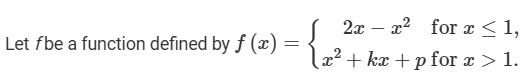
\includegraphics[width=0.7\linewidth]{Q1_1}
		\begin{parts}
			\part For what values of $k$ and $p$ will $f$ be continuous and differentiable at $x = 1$?
			\part For the values of $k$ and $p$ found in part (a), on what interval or intervals is $f$ increasing?
			\part Using the values of $k$ and $p$ found in part (a), find all points of inflection of the graph of $f$. Support your conclusion.
		\end{parts}
		
		\begin{solution}
		\begin{parts}
			\part 
			Definition of continuity of $f$ at $x=1$:
			\begin{gather}
				\lim_{x \to 1^{+}} f(x) = \lim_{x \to 1^{-}} f(x) = f(1) \\
				\lim_{x \to 1^{+}} f(x) = 1^2 + 1k + p \\
				\lim_{x \to 1^{-}} = f(1) = 2(1) - (1)^2 = 2 - 1 = 1  \\
				\textit{Therefore, } 1 = 1 + k +p \implies \boxed{-k = p} \label{eq:k_p_1}		
			\end{gather}
			Differentiate $f$ with respect to $x$ (needed for next step):
			\begin{align}
				f^\prime(x) &= \begin{cases}
					\frac{d}{dx} (2x-x^2) & \text{ for } x \leq 1, \\
					\frac{d}{dx} (x^2+kx+p) & \text{ for } x > 1.
				\end{cases}	\\
				f^\prime(x) &= \begin{cases}
					2-2x & \text{ for } x \leq 1, \\
					2x+k+0 & \text{ for } x > 1.
				\end{cases}
			\end{align}
			Definition of differentiability of $f$ at $x=1$:
			\begin{gather}
				\lim_{x \to 1^{+}} f^{\prime}(x) = \lim_{x \to 1^{-}} f^{\prime}(x) = f^{\prime}(1) \\
				\lim_{x \to 1^{-}} f^{\prime}(x) = f^{\prime}(1) = 2-2(1) = 0 \\
				\lim_{x \to 1^{+}} f^{\prime}(x) = 2(1) + k \\
				\textit{Therefore, } 2+k = 0 \implies \boxed{-2 = k} \label{eq:k_2}
			\end{gather}
			Conclusion:
			Using Equations \ref{eq:k_2} and \ref{eq:k_p_1}:
			\begin{gather}
				-2 = k \quad -k = p \\
				-(-2) = p \implies p = 2 \\
				\boxed{\textit{Therefore, } k = -2 \text{ and } p = 2}			
			\end{gather}
			
		\part $f^\prime(x) > 0$ when $f$ is increasing.
		$$f^\prime(x) = \begin{cases}
			2 - 2x & \text{ for } x \leq 1, \\
			2x - 2 & \text{ for } x > 1.
			\end{cases}
		$$ \\
		On $x \leq 1$, set $f^\prime(x) = 0$:
		$$2-2x = 0 \implies 2=2x \implies 1=x$$
		Sign chart for $2-2x$: (Only applies to $f^\prime(x)$ on $x>1$)
		$$\sgchart {1} {2-2x: +-}$$
		On $x > 1$, set $f^\prime(x) = 0$:
		$$2x-2 = 0 \implies 2x=2 \implies x=1$$
		Sign chart for $2x-2$: (Only applies to $f^\prime(x)$ on $x>1$)
		$$\sgchart {1} {2x-2: -+}$$
		Combined sign chart for $f^\prime(x)$:
		$$\sgchart {1} {f^\prime(x):++}$$
		Conclusion:
		$$ \textit{Therefore, } f(x)\text{ is increasing when } x \neq 1 $$
		$$\text{because } f^\prime(x) \text{ is positive on those regions. } (\text{At } x=1, f^\prime(x) = 0.)$$
		$$f \text{ is continuous at } x=1, \text{ so } \boxed{ f(x) \text{ is increasing on } (-\infty, \infty). }$$
		\part Inflection points are where $f^{\prime\prime}$ changes signs.
		$$f^{\prime\prime}(x) = \begin{cases}
			\frac{d}{dx} (2 - 2x) = -2 & \text{ for } x \leq 1, \\
			\frac{d}{dx} (2x - 2) = 2 & \text{ for } x > 1.
		\end{cases}
		$$
		Sign chart of $f^{\prime\prime}(x)$:
		$$\sgchart {~1} {f(x): -+}$$ 
		\textit{Therefore,} $f^{\prime}(x)$ has an inflection point at $x=1$.
		$$f(1) = 1 \quad\quad \boxed{\text{Inflection Point: } (1,1)}$$
		\end{parts}
		\end{solution}
		
		\question Consider the curve given by $x^2-xy+2y^2=7$.
		\begin{parts}
			\part Show that $\frac{dy}{dx} = \frac{y-2x}{4y-x}$
			\part Determine the $y$-coordinate of each point on the curve at which the line tangent to the curve at that point is vertical. Justify your answer.
			\part Find $\frac{d^2y}{dx^2}$ in terms of $x$, $y$, and $\frac{dy}{dx}$. The line tangent to the curve at the point $(1,2)$ is horizontal. Determine whether the curve is concave up or concave down at the point $(1,2)$.
		\end{parts}
		
		\begin{solution}
			\begin{parts}
				\part 
				\begin{align}
					\frac{d}{dx} (x^2 - xy + 2y^2) &= 7 \\
					2x - (xy^\prime + y) + 4yy^\prime &= 0 \\
					2x - xyy^\prime - y + 4yy^\prime &= 0 \\
					2x - y &= y^\prime(x-4y) \\
					\frac{2x-y}{x-4y} &= y^\prime = \frac{dy}{dx} = \frac{y-2x}{4y-x} 
				\end{align}
				\part Vertical tangent lines have undefined slope. \\
				Therefore, $\frac{dy}{dx}$ will be undefined $\iff$ the tangent line at the point is vertical. \\
				($\iff$ means 'if and only if') \\
				\begin{align}
					4y-x = 0 & \text{ makes } \frac{dy}{dx} \text{ undefined.} \\
					4y   = x
				\end{align}
				So,
				\begin{align}
					7 &= (4y)^2 - (4y)y + 2y^2  \\
					7 &= 16y^2 - 4y^2 + 2y^2  \\
					7 &= 14y^2  \\
					y^2 &= \frac{1}{2} \\
					y &= \boxed{\pm \frac{1}{\sqrt{2}} }
				\end{align}
				
				\part
				\begin{align}
					\frac{d^2y}{dx^2} &= \frac{d}{dx} \left( \frac{dy}{dx} \right) = \frac{d}{dx} \left( \frac{y-2x}{4y-x} \right) \\
					&= \frac{ \left( \nicefrac{d}{dx} \left( y-2x \right) \right) \left( 4y - x \right) - \left( \nicefrac{d}{dx} \left( 4y - x \right) \right) \left( y-2x \right) } { \left( 4y - x \right)^2 } \\
					&= \frac{ \left( y^\prime - 2 \right) \left( 4y - x \right) - \left( 4y^\prime - 1 \right) \left( y-2x \right) } { \left( 4y - x \right)^2 }
				\end{align}
				$y^\prime = 0$ at $(1,2)$ since the tangent to the curve is vertical.
				\begin{align}
					\frac{d^2y}{dx^2} \bigg{|}_{(1,2)} &= \frac{(-2)(4(2)-1)-(-1)(2-2(1))}{(4(2)-1)^2}
													   &= \frac{-2(7)-0}{7^2} = -\frac{2}{7}
				\end{align}
				$$\boxed{ \text {Since } \frac{d^2y}{dx^2} \text{ is negative at $(1,2)$, the curve is concave down at $(1,2)$.}}$$
			\end{parts}
		\end{solution}
		
		\question Particle $P$ moves along the $y$-axis so that its position at time $t$ is given by $y(t) = 4t - \frac{2}{3}$ for all times $t$. A second particle, particle, moves along the-axis so that its position at time $t$ is given by $x(t) = \frac{\sin(\pi t)}{2-t}$ for all times $t \neq 2$.
		
		\begin{parts}
			\part As time $t$ approaches $2$, what is the limit of the position of particle $Q$? Show the work that leads to your answer.
			\part Show that the velocity of particle $Q$ is given by $v_Q(t) = \frac{2\pi\cos(\pi t)-\pi t \cos (\pi t) + \sin(\pi t)}{(2-t)^2}$ for all times. 
			\part Find the rate of change of the distance between particle $P$ and particle $Q$ at time $t=\frac{1}{2}$. Show the work that leads to your answer.
		\end{parts}
		
		\begin{solution}
			\begin{parts}
				\part \begin{align}
					\lim_{t\to2} \left( \sin \left( \pi t \right) \right) &= \sin \left( 2\pi \right) = 0 \\
					\lim_{t\to2} \left( 2 - t \right) &= 0
				\end{align}
				Since $\frac{\lim_{t\to2} \left( \sin \left( \pi t \right) \right)}{\lim_{t\to2} \left( 2 - t \right)}$ approaches an indeterminate form (\nicefrac{0}{0}), L'Hôpital's rule can be applied.
				\begin{align}
					\lim_{t\to2} \left( \nicefrac{d}{dt} \left( \sin \left( \pi t \right) \right) \right) &= \lim_{t\to2} \left( \pi \cos \left( \pi t \right) \right) = \pi \cos(2\pi) = \pi \\
					\lim_{t\to2} \left( \nicefrac{d}{dt} \left( 2 - t \right) \right) &= \lim_{t\to2} \left( -1 \right) = -1 \\
					\therefore \lim_{t\to2} (x(t)) &= \frac{\pi}{-1} = \boxed{-\pi}
				\end{align}
				
				\part \begin{align}
				\frac{d}{dt} \left( x(t) \right) &= v_Q(t) \\
				\frac{d}{dt} \left( \frac{\sin(\pi t)}{2-t} \right) &= \frac{ (\nicefrac{d}{dt}(\sin(\pi t))) (2-t) - (\nicefrac{d}{dt} (2-t))(\sin (\pi t)) }{(2-t)^2} \\
				&= \frac{ \pi \cos(\pi t) (2-t) - (-1)(\sin (\pi t)) }{(2-t)^2} \\
				&= \frac{2\pi\cos(\pi t)-\pi t \cos (\pi t) + \sin(\pi t)}{(2-t)^2}
				\end{align}
				
				\part
					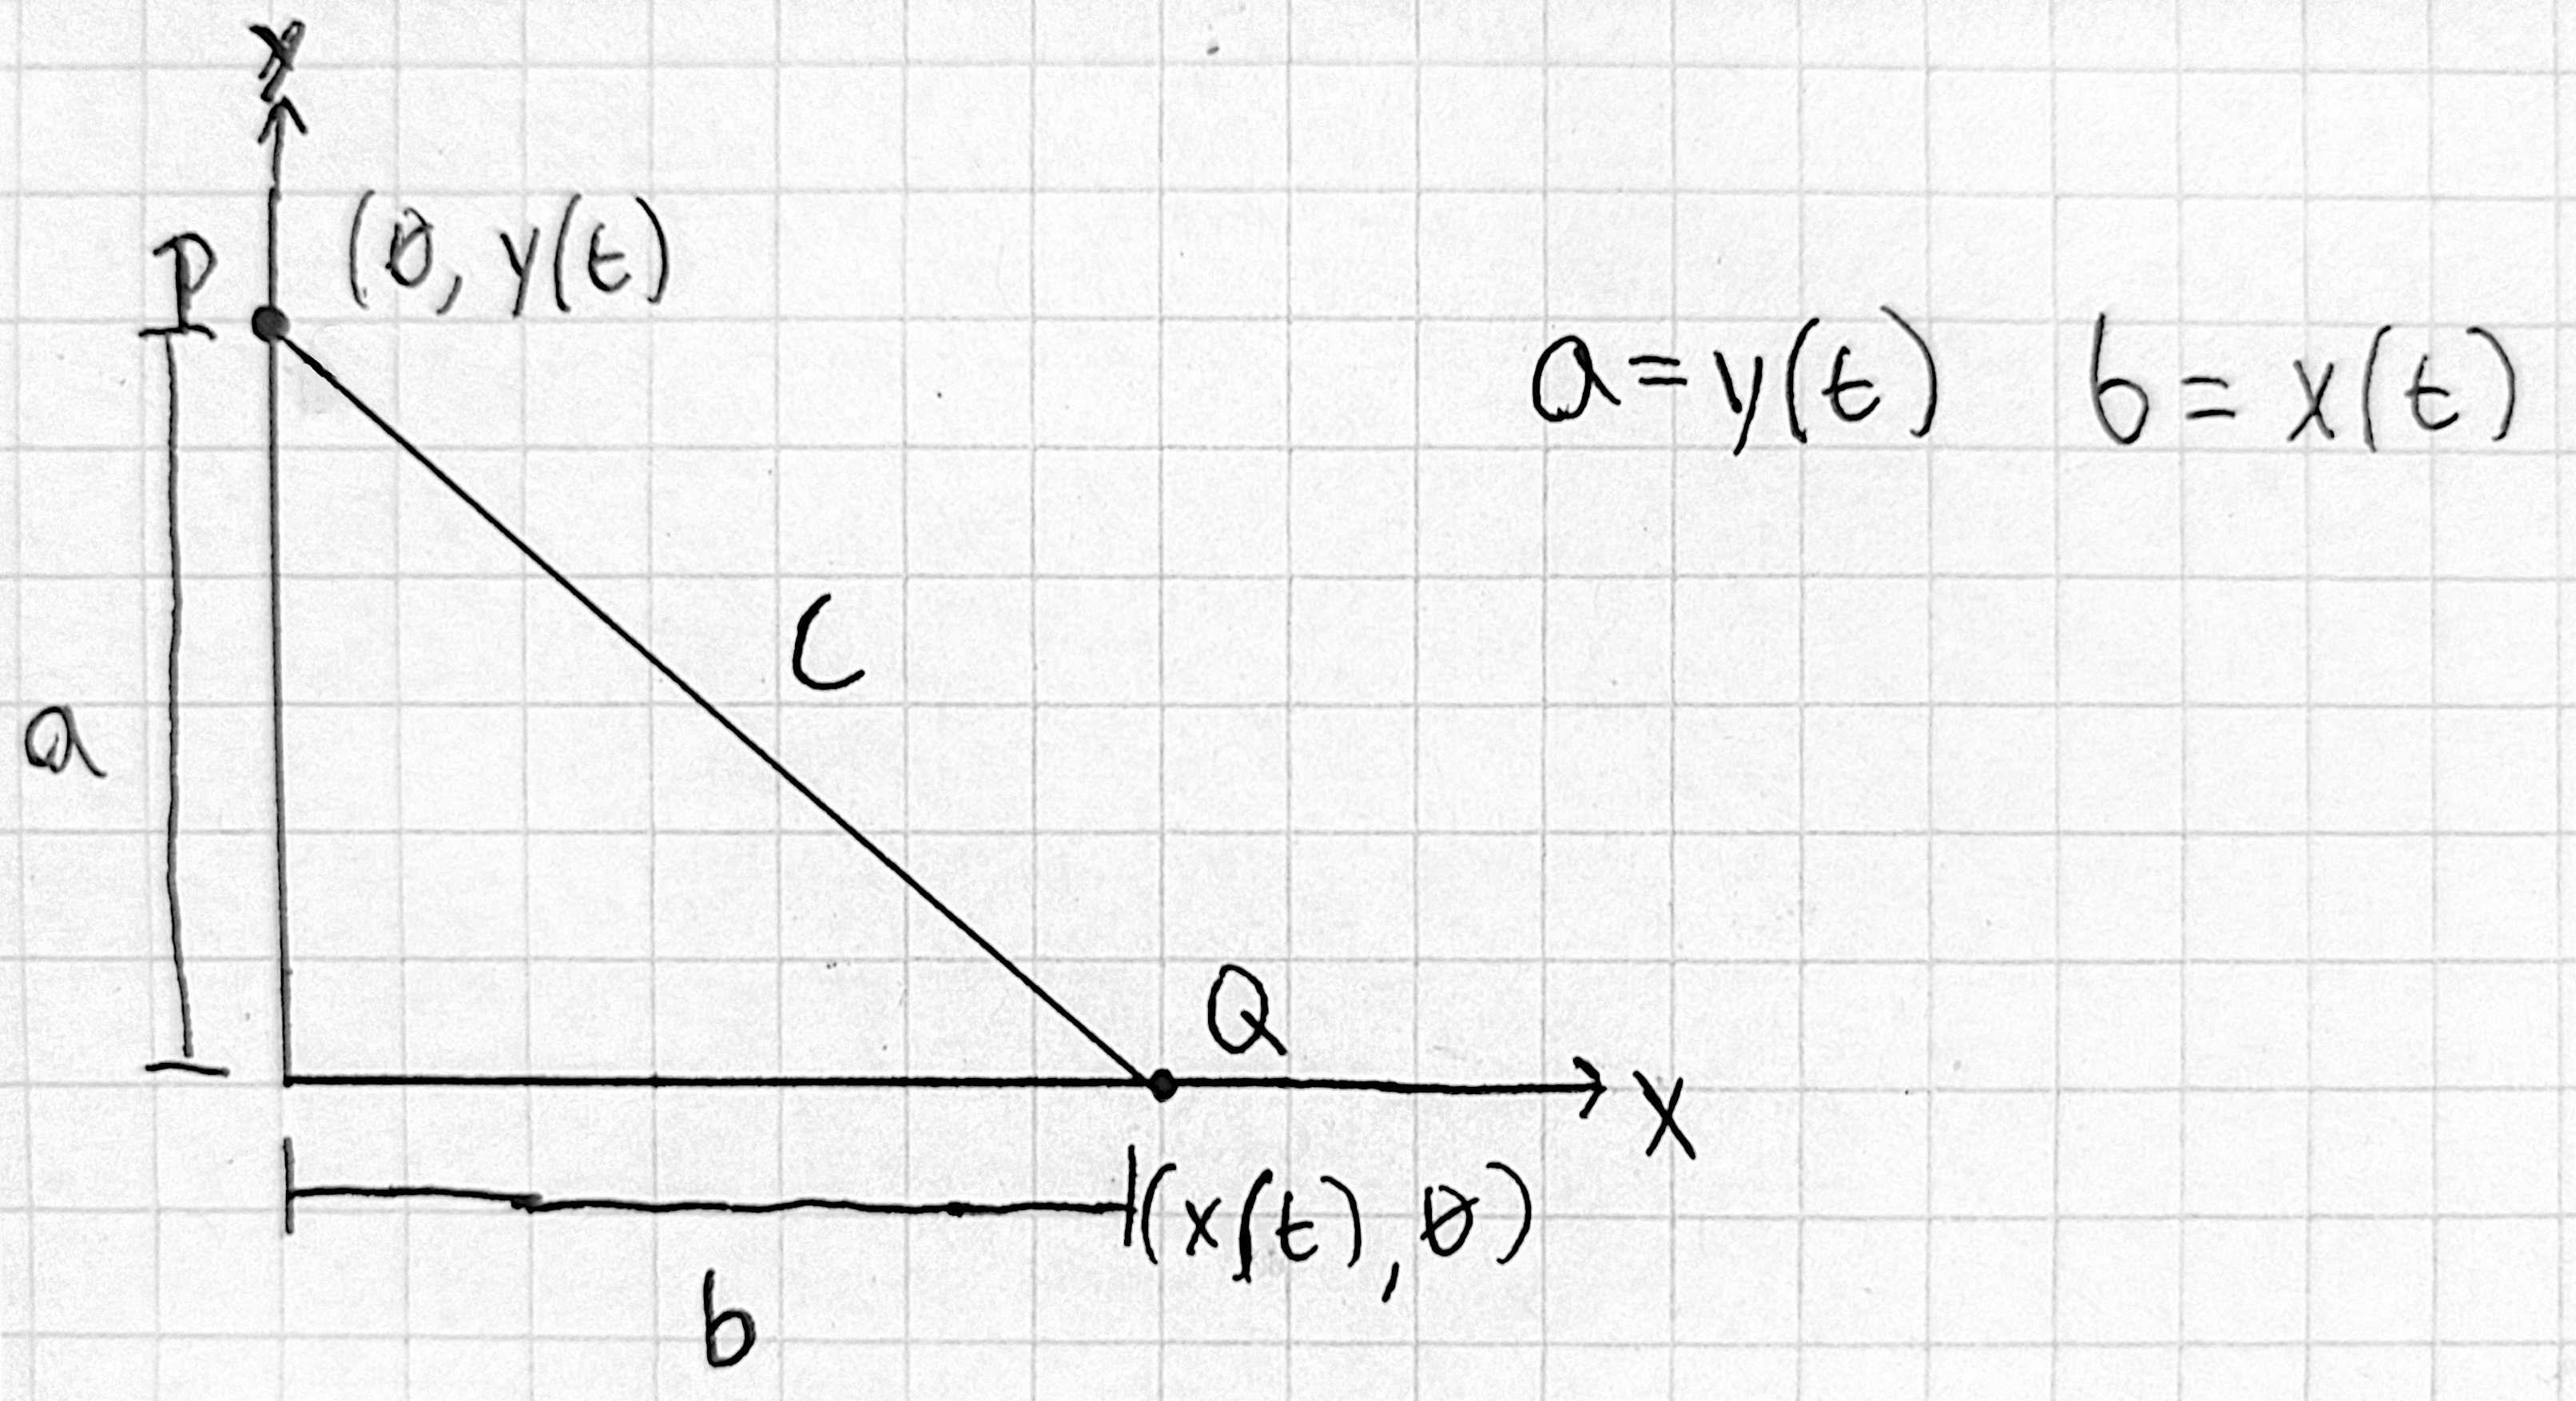
\includegraphics[width=0.7\linewidth]{Q3c_1}
					\begin{gather}
						c^2 = a^2+b^2 \\
						c = \sqrt{a^2+b^2} \\ \\
						2c\frac{dc}{dt} = 2a\frac{da}{dt} + 2b\frac{db}{dt} \\
						\frac{dc}{dt} = \frac{a\frac{da}{dt} + b\frac{db}{dt}}{c} \\ 
						\uparrow \text{Main rate equation} \uparrow \\ \\
						a = y(t) = 4t-\frac{2}{3} \\
						\frac{da}{dt} = 4 \\ \\
						b = x(t) = \frac{\sin(\pi t)}{2-t} \\
						\frac{db}{dt} = \frac{(\pi \cos (\pi t))(2-t)-(-1)(sin(\pi t))}{(2-t)^2} 
					\end{gather}
				Now, find all of those variables when $t=\frac{1}{2}$
				\begin{gather}
					a|_{t=\nicefrac{1}{2}} = 4(\nicefrac{1}{2}) - \nicefrac{2}{3} = 2 - \nicefrac{2}{3} = \nicefrac{4}{3} \\
					b|_{t=\nicefrac{1}{2}} = \frac{\sin(\nicefrac{\pi}{2})}{2-\nicefrac{1}{2}} = \frac{1}{\nicefrac{3}{2}} = \frac{2}{3} \\
					\frac{da}{dt}\bigg{|}_{t=\nicefrac{1}{2}} = 4 \\
					\frac{db}{dt}\bigg{|}_{\nicefrac{1}{2}} = \frac{(\pi \cos (\nicefrac{\pi}{2}))(2-\nicefrac{1}{2}) + (sin(\nicefrac{\pi}{2}))}{(2-\nicefrac{1}{2})^2} = \frac{4(\pi(0)(\nicefrac{3}{2}) + 1)}{9} = \frac{4}{9} \\
					c|_{t=\nicefrac{1}{2}} = \sqrt{a^2 + b^2} = \sqrt{(\nicefrac{4}{3})^2 + (\nicefrac{2}{3})^2} = \sqrt{\nicefrac{20}{3}}
 				\end{gather}
 				Finally, plug all of those into our main rate equation:
 				$$\frac{dc}{dt}\bigg{|}_{t=\nicefrac{1}{2}}  = \frac{(\nicefrac{4}{3})(4) + (\nicefrac{2}{3})(\nicefrac{4}{9})}{\sqrt{\nicefrac{20}{3}}}$$
			\end{parts}
		\end{solution}
		
		\question Let $f$ be the function given by $f(x) = 2xe^{2x}$. \\
		Find the absolute minimum value of $f$. Justify that your answer is an absolute minimum.
		\begin{solution}
			All absolute minimums must also be relative minima. \\
			\quad At Relative minima of $f$, the derivative, $f^\prime$ changes from negative to positive.
			Find $f^\prime(x)$
			\begin{align}
				f^\prime(x)	&= 2(1(e^{2x}) + x(2e^{2x})) \\
							&= 2e^{2x} + 2xe^{2x} \\
							&= 2e^{2x}(1+x)
			\end{align}
			Set $f^\prime(x) = 0$ and solve:
			$$ 2e^{2x}(1+x) $$
			\begin{align}
				2e^{2x} = 0 		\ \   &| \ \  (1+x) = 0 \\
				\ln (e^2x) = 0 		\ \   &| \ \ x = -1 \\
				\text{no solution	\ \ } &| \ \ 
			\end{align}
			Sign chart of $f^\prime(x)$:
			$$\sgchart{-1}{f^\prime(x):-+}$$
			Find end behavior of $f(x)$:
			\begin{align}
				\lim_{x\to  \infty} \left( 2x e^{2x} \right) &= \lim_{x\to  \infty} \left( e^{2x} \right) &= \infty
				\lim_{x\to -\infty} \left( 2x e^{2x} \right) &= \lim_{x\to -\infty} \left( e^{2x} \right) &= 0
			\end{align}
			Conclusion: \\
			Since $x=-1$ is the only relative minima and is less than the $\lim_{x\to \pm \infty} (f(x))$, it is the absolute minimum of $f(x)$.
			$$f(-1) = 2(-1)e^{2(1)}= -2e^{2}$$
			The absolute minimum of $f(x)$ is $\boxed{f(-1) =-2e^{2}}$
		\end{solution}
		\setcounter{question}{13}
		\question 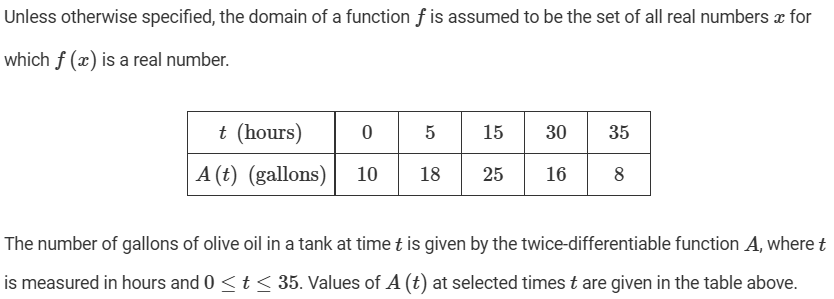
\includegraphics[width=1\linewidth]{chrome_znbfVtBkrt}
		\begin{parts}
			\part Use the data in the table to estimate the rate at which the number of gallons of olive oil in the tank is changing at time $t=10$ hours. Show the computations that lead to your answer. Indicate units of measure.
			\part For $0 \leq t \leq 30$, is there a time $t$ at which $A^\prime(t) = \frac{1}{5}$? Justify your answer.
			\part The number of gallons of olive oil in the tank at time $t$ is also modeled by the function $G$ defined by $G(t) = 5t - \frac{2}{3} (t+9)^{\frac{3}{2}} +28$, where $t$ is measured in hours and $0 \leq t \leq 35$. Based on the model, at what time $t$, for $0 \leq t \leq 35$, is the number of gallons of olive oil in the tank an absolute maximum? Justify your answer.
		\end{parts}
		
		\begin{solution}
			\begin{parts}
				\part $$A^\prime(t) \approx \frac{A(30)-A(15)}{30-15} = \frac{16-25}{30-15} = - \frac{9}{15} = - \frac{3}{5}$$
				\part On $0 \leq t \leq 30$, the AROC can be found as follows:
				$$\frac{A(30)-A(0)}{30-0}=\frac{16-10}{30}=\frac{6}{30}=\frac{1}{5}$$
				Since $A$ is twice-differentiable $\implies A$ is differentiable $\implies A$ is continuous.  \\
				Therefore, by MVT, there is a value $c$ in $(0,30)$ where $A^\prime(c) = \frac{A(30)-A(0)}{30-0}=\frac{1}{5}$.
				\part Coming Soon™
				\part Coming Soon™
			\end{parts}
		\end{solution}
	\end{questions}
\end{document}